% !TEX root = ../../presentation.tex
% Meta: Struktur

\begin{slide}{Struktur}
  \begin{columns}
    \begin{column}{0.45\textwidth}
      \small
      \pause
      \textbf{1 Assembler Simulator}

      \pause
      \vspace{0.5cm}
      \begin{tabular}{ll}
        \textbf{Zutat} & \textbf{Menge}\\
        \toprule
        Arch & 3-4P \\
        Core & 2-3P \\
        Parser & 2P \\
        GUI & 3P    \\
        \pause
        Projektleiter & 1P
      \end{tabular}
    \end{column}
    \begin{column}{0.55\textwidth}
      \pause
      \begin{tikzpicture}
        \node [inner sep=0pt ]at (0, 0) {%
          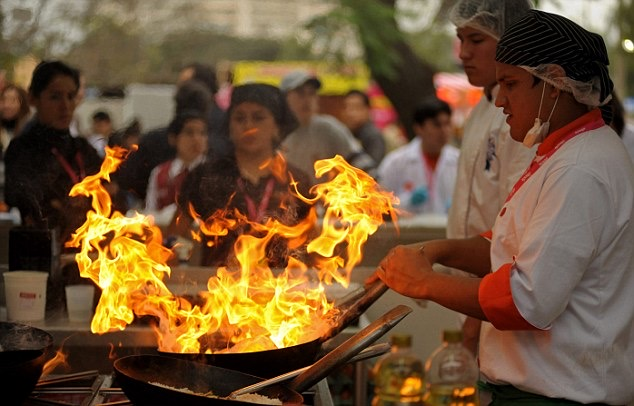
\includegraphics[width=5.5cm]{cooking}
        };

        \draw [white, rounded corners=0.1cm, line width=0.1cm]
          (current bounding box.north west) --
          (current bounding box.north east) --
          (current bounding box.south east) --
          (current bounding box.south west) --
          cycle;
      \end{tikzpicture}
    \end{column}
  \end{columns}
\end{slide}
